\documentclass[11pt]{article}
\usepackage[margin=1in]{geometry}
\usepackage[T1]{fontenc}
\usepackage{times}
\usepackage[utf8]{inputenc}
\usepackage{microtype}
\usepackage{amsmath,amssymb}
\usepackage{booktabs}
\usepackage{graphicx}
\usepackage{xcolor}
\usepackage[numbers,sort&compress]{natbib}
\usepackage[hidelinks]{hyperref}
\renewcommand{\topfraction}{0.9}
\renewcommand{\bottomfraction}{0.8}
\renewcommand{\textfraction}{0.1}
\renewcommand{\floatpagefraction}{0.85}
\setlength{\textfloatsep}{12pt plus 2pt minus 4pt}

\title{Knowledge or Capacity? Lessons from a 2\,MB\\ On-Device Classifier for What Is Playing}
\author{Xin Gao}
\date{}

\begin{document}
\maketitle

\begin{abstract}
We study how to tell what is playing (the content type, one of ten music genres, and whether a video is entertainment or informational) from text metadata alone: the title, the artist or channel, the site and the duration, for titles in English, Japanese and Chinese, entirely on the device. A 2.1\,MB hashed character $n$-gram linear model with deterministic site rules and an updatable artist table runs in under 1\,ms per item, and its TypeScript port reproduces the Python reference exactly. On 383 real titles collected from live charts and trending pages it is fully right on 84.9\% of items, against 95.3\% for a large language model reading the same four fields. Two negative results suggest where the gap lies: training the linear model on the large model's labels did not help, and a 107M-parameter multilingual transformer reached 84.1\%. The evidence points to missing knowledge rather than missing capacity: genre accuracy is 90.5\% for artists the system has seen but 47.8\% for unseen ones, where the large model still reaches 87.0\%. A confidence-gated hybrid that hands the least confident 31.9\% of items to the large model is fully right on 95.6\%, on par with sending everything. We also find that validation data written by a large language model overstated real-world genre accuracy by 10.5 to 15.3 points.
\end{abstract}

\section{Introduction}
\label{sec:intro}

Applications that react to what a person is watching or listening to, such as media players, recommenders and desktop companions, need to know what kind of item is playing. Music information retrieval has studied genre recognition for more than two decades, mostly from the audio signal and from rich context such as web pages and collaborative tags \citep{tzanetakis2002musical,schedl2014music}. A browser extension or a desktop application, however, usually sees only the text metadata that the page or the operating system exposes: a title, an artist or channel name, the site, and sometimes a duration. Capturing audio needs extra permissions and power, and sending every title to a server raises privacy and availability concerns. This paper studies the text-only, on-device version of the problem.

Our setting is a companion application, a browser extension with planned desktop versions, that shows an animated character reacting to the media being played. For each item it must decide the content type (music, video, live stream or podcast), one of ten coarse genres for music, and whether a video is entertainment or informational. Titles come in English, Japanese and Chinese, often mixed within one string. The same model must run in a browser-extension service worker, in Swift and in C\#, give the same output in each, fit comfortably in an extension package, and take well under a few milliseconds per item. It may abstain, because a wrong answer only shows a mismatched character.

Two families of tools fit parts of this specification. Linear classifiers over hashed n-gram features are small, fast and easy to port \citep{joulin2017bag,weinberger2009feature}, and can be compressed further by quantisation \citep{joulin2016fasttextzip,gholami2021survey}. Large language models can label text with little or no task-specific training \citep{gilardi2023chatgpt,wang2021want}, although careful prompting may be needed to match fine-tuned classifiers \citep{sun2023text}, and models such as the DeepSeek family \citep{deepseekai2024deepseekv3} cannot run inside an extension. Large language models can also write labelled training data \citep{li2023synthetic,long2024llmsdriven}, which makes a cheap data pipeline possible but raises the question of how such a pipeline should be evaluated.

The difficulty is that a media title carries little linguistic signal, and its genre is largely decided by facts about the artist or the work: which anime a song belongs to, which producer made a track, what a meme refers to. A small model learns surface patterns from a fixed training set, so when the artist or the work is absent from that set it has nothing to go on. It is therefore unclear how far a tiny on-device model can go, what limits it, and whether a stronger on-device learner, trained on a large model's labels or built on a small multilingual transformer, closes the gap to a large language model. We study these questions for one task, with a system that combines deterministic site rules, a hashed character $n$-gram linear model and an updatable artist-to-genre table. Our hypothesis is that the remaining errors reflect missing world knowledge rather than missing capacity.

Our contributions are:
\begin{itemize}
    \item An openly released, trilingual (English, Japanese, Chinese), text-only media classifier of 2.1\,MB that runs in under 1\,ms per item and is fully right on 84.9\% of 383 real titles, against 95.3\% for a large language model given the same text.
    \item Evidence that the gap is mainly missing knowledge: genre accuracy collapses on unseen artists, while training on the large model's labels and a 107M-parameter multilingual encoder both fail to improve real-world accuracy.
    \item A confidence-gated hybrid that hands 31.9\% of items to the large model and reaches 95.6\%, on par with sending every item.
    \item A measurement showing that validation data written by a large language model overstated real-world genre accuracy by 10.5 to 15.3 points.
\end{itemize}

\section{Related Work}
\label{sec:related}

\paragraph{Music and media classification from text and metadata.}
Genre recognition has mainly been studied from audio \citep{tzanetakis2002musical}, with text playing a supporting role. Lyrics are the most studied text source: early work used rhyme and stylistic features \citep{mayer2008rhyme}, later work combined lyrics analysis with classification \citep{fell2014lyrics}, and hierarchical attention networks classify complete lyrics into up to 117 genres \citep{tsaptsinos2017lyrics}. Multimodal approaches combine audio, album reviews and cover images for multi-label genre tagging \citep{oramas2017multilabel}. Other work uses context outside the recording, such as social tags \citep{lamere2008social} and web-based data about artists \citep{knees2004artist}. For video, text metadata and user comments have been used to assign categories \citep{filippova2011improved}. These methods assume access to lyrics, reviews, tags, comments or web search results, none of which a media player's metadata provides. In our literature search we found little work on genre classification from short titles in mixed English, Japanese and Chinese. Our input is limited to the title, artist, site and duration, and we keep artist knowledge in an explicit table that can be updated without retraining, rather than expecting the model to learn it.

\paragraph{Efficient linear text classifiers and feature hashing.}
Linear models over word and n-gram features remain strong baselines for sentiment and topic classification \citep{wang2012baselines}. fastText showed that such a model is often on par with deep classifiers in accuracy while being many orders of magnitude faster to train and evaluate \citep{joulin2017bag}. Subword character n-grams improve representations of rare words \citep{bojanowski2017enriching}, and product quantisation reduces model memory by about two orders of magnitude with a small accuracy loss \citep{joulin2016fasttextzip}. Feature hashing maps an unbounded feature space into a fixed number of buckets with a bounded effect of collisions \citep{weinberger2009feature}. Character-level models avoid word segmentation, which matters for Chinese and Japanese: character n-gram language models categorise text in Chinese, Japanese, English and Greek without language-specific preprocessing \citep{peng2003language}, and character-level convolutional networks are competitive on large datasets \citep{zhang2015character}. The limitation for our task is that these models capture surface patterns but cannot know entity facts, such as an artist's genre, beyond what appears in their training data. We adopt the hashed character n-gram linear model for its size, speed and portability, and supply that knowledge through site rules and the artist table.

\paragraph{Compact multilingual transformers and knowledge distillation.}
Multilingual pretrained encoders such as XLM-R \citep{conneau2020unsupervised} handle many languages and scripts in one model. Knowledge distillation compresses what a large model or ensemble has learned into a smaller model \citep{hinton2015distilling}, producing compact encoders such as DistilBERT \citep{sanh2019distilbert}, MiniLM \citep{wang2020minilm} and MiniLMv2 \citep{wang2021minilmv2}, and even single-layer BiLSTM students \citep{tang2019distilling}; the multilingual MiniLMv2 encoder we compare against is distilled from XLM-R Large. In multilingual models most parameters sit in the vocabulary embeddings, so trimming the vocabulary to the target languages can remove up to 45\% of the parameters \citep{abdaoui2020load}. With large language models, the teacher's labels or rationales can train small task models \citep{hsieh2023distilling,wang2021want}, and its annotations can match or exceed crowd workers \citep{gilardi2023chatgpt}. Entirely synthetic training sets are another route \citep{long2024llmsdriven}, but their usefulness falls as the task becomes more subjective \citep{li2023synthetic}. We hypothesise that distillation transfers decision rules that can be learned from the input, but cannot place entity knowledge into a student whose capacity or input representation has no room for it.

\paragraph{Cascades, selective prediction and model routing.}
A classifier with a reject option abstains when its confidence is low, trading coverage for error \citep{chow1970optimum}. Selective classification makes this trade-off controllable for deep networks with a guaranteed risk level \citep{geifman2017selective}, and works only as well as the underlying confidence estimates, which modern networks often get wrong \citep{guo2017calibration}. Cascades send an input to a larger model only when a smaller one is unsure; in NLP, cascading has been shown to reduce computation and, in some settings, improve accuracy over the largest model alone \citep{varshney2022model}. For large language models, FrugalGPT learns which combination of models to query for each input, reducing cost while keeping or improving accuracy \citep{chen2023frugalgpt}, and hybrid routing assigns each query to a small edge model or a large cloud model based on predicted difficulty \citep{ding2024hybrid}. This work mostly targets the serving cost of generative models, where the small model is itself a language model. Our case differs in scale and purpose. The local model is a 2.1\,MB linear classifier that runs privately and offline, and the gate exists so that most items never leave the device.

\section{Method}
\label{sec:method}

Figure~\ref{fig:pipeline} summarises the system. Everything up to the thresholds runs on the device; the hand-off to a large language model is optional.

\begin{figure}[t]
  \centering
  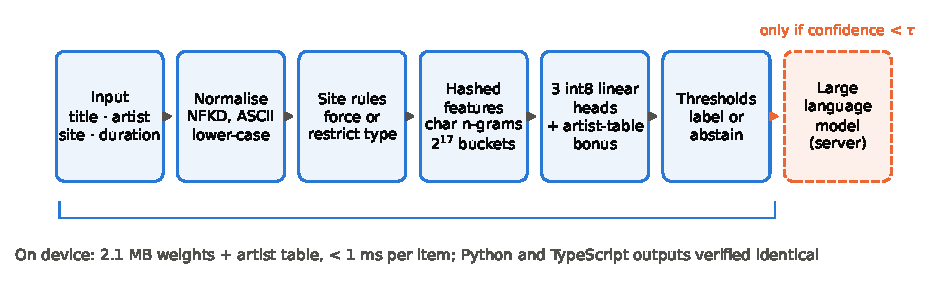
\includegraphics[width=\linewidth]{figures/fig_pipeline_overview.pdf}
  \caption{The classification pipeline. Everything left of the dashed branch runs on the device; items whose combined confidence falls below the threshold $\tau$ can optionally be handed to a server-side large language model that sees the same four fields.}
  \label{fig:pipeline}
\end{figure}

\subsection{Task and Labels}
\label{sec:task}

An item is a tuple (title, artist or channel, site host, duration), where the duration may be missing. The system predicts a \emph{type} in \{music, video, live, podcast\}; for music, a \emph{genre} in \{rock, western-pop, jpop, anime, cpop, electronic, lofi, classical, hiphop, other\}; and for video, a \emph{video class} in \{ent, info\} (entertainment versus informational). The genres are deliberately coarse and product-driven: western-pop includes K-pop and R\&B, anime includes Vocaloid, VTuber and game music, lofi includes ambient and sleep sounds, classical includes film scores, and other collects jazz, country, folk, enka and children's songs. A written label guide fixes the hard boundaries: meme videos, MAD videos (fan-edited music videos) and remixes and anime episodes or clips are video/ent; anime openings, endings, character songs and soundtracks are music/anime; idol music videos and concerts are music/jpop, idol variety shows are video/ent, idol live streams are live and idol radio is podcast. Any head may abstain, in which case the application shows a generic character.

\subsection{Features and Model}
\label{sec:model}

\paragraph{Normalisation.} Text is normalised with Unicode NFKD, combining marks (U+0300--U+036F) are dropped, only ASCII letters are lower-cased so that every runtime behaves identically, and whitespace (including the ideographic space) is collapsed. The site is the host name without a leading \texttt{www.} or \texttt{m.}, mapped through a small alias table.

\paragraph{Hashed features.} For the title and the artist separately we take the first 160 Unicode code points, add boundary markers, and emit character $n$-grams for $n = 1,\dots,4$, tagged by field, plus untagged copies for $n \ge 2$ that are shared between the two fields. Character $n$-grams need no word segmentation, which matters for Chinese and Japanese. We also emit ASCII word unigrams and adjacent-word bigrams, the site, a duration bucket (unknown, live, and seven ranges from under 60\,s to over an hour) and the site~$\times$~duration pair. Each feature string is hashed with 32-bit FNV-1a over its UTF-8 bytes and masked to $B = 2^{17} = 131{,}072$ buckets, the hashing trick \citep{weinberger2009feature}. The input is the set $S$ of distinct bucket indices.

\paragraph{Three linear heads.} A type head ($K=4$), a genre head ($K=10$, trained on music rows) and a video-class head ($K=2$, trained on video rows) share the hashed input. For head $h$ with weights $W_h \in \mathbb{R}^{K_h \times B}$ and bias $b_h$,
\begin{equation}
  z_h = b_h + \frac{1}{\sqrt{|S|}} \sum_{i \in S} W_h[:, i], \qquad p_h = \operatorname{softmax}(z_h).
  \label{eq:logits}
\end{equation}
Each head is a multinomial logistic regression trained with L-BFGS \citep{liu1989limited} in scikit-learn \citep{pedregosa2011scikitlearn}, with inverse regularisation $C = 30$ and balanced class weights. For each training row we add one perturbed copy in which, independently, the artist is removed (probability 0.35), a known duration is set to unknown (0.5) and the site is removed (0.15); the copy is kept if at least one field changed. This teaches the model to cope with missing fields. The genre head also sees artist-only and title-only rows built from the artist table (Section~\ref{sec:rules}).

\paragraph{Quantisation and portability.} Each head is quantised to symmetric int8 with one scale per head, $\mathrm{scale}_h = \max |W_h| / 127$; biases stay in float32. The weights occupy 2,097,256 bytes. Inference is a table lookup, a sum and a softmax, which takes a few dozen lines in each language. A shared file of test vectors (inputs with expected outputs to $10^{-9}$, plus a hash of the feature indices) specifies the behaviour of every port; the TypeScript runtime matches the Python reference on all 559 vectors, while the Swift and C\# ports have been written but not yet compiled or run.

\subsection{Site Rules, Artist Table and Abstention}
\label{sec:rules}

\paragraph{Site rules.} What the platform already knows is used directly: music-only sites force the type to music, podcast sites force podcast, film and course sites restrict the type softmax to video, and live streams restrict it to music or live. A category reported by the player (for example a podcast episode URL) overrides the model.

\paragraph{Artist table.} Genre depends mostly on who the artist is, so this knowledge lives in an explicit, updatable table from normalised artist names and aliases to genres (25,826 keys in the shipped model). If the artist field, or one of its segments split on separators such as ``/'', ``\&'' or ``feat'', matches the table, we add a bonus $\beta_a$ to that genre's logit; otherwise, a matching title segment adds $\beta_t$ (the shipped model uses $\beta_a = \beta_t = 3$). A bonus rather than an override lets cues in the title (for example an anime opening marker) still change the answer. Conflicts between sources are resolved by a fixed priority: curated lists, then chart-derived labels, then training-data votes.

\paragraph{Abstention and confidence.} A head abstains below its threshold (type 0.4, genre 0.3, video class 0.5 in the shipped model, tuned on the real development split). For hand-off we define a combined confidence $c = \min(p_\text{type}, p_\text{genre})$ for music, $c = \min(p_\text{type}, p_\text{vclass})$ for video, $c = p_\text{type}$ for live and podcast, and $c = 0$ whenever any head abstains.

\subsection{Large-Model Teacher and Hybrid}
\label{sec:hybrid}

As a reference and teacher we use DeepSeek V4.1 Flash, a model of the DeepSeek family for which no separate technical report exists (we cite the V3 report \citep{deepseekai2024deepseekv3} for the family), self-hosted and queried with temperature 0 and JSON output, 20 items per request. It receives exactly the same four fields and the label guide as its system prompt, so it has no additional input to draw on; any advantage must come from what it has learned about the same text. We use it in three ways: as an upper reference on the same text; as a teacher for distillation, by labelling unlabelled real titles and auditing existing labels (Section~\ref{sec:distill}); and in a \emph{hybrid}, where an item is sent to it only when the small model's combined confidence is below a threshold $\tau$.

\section{Experimental Setup}
\label{sec:setup}

\subsection{Data}
\label{sec:data}

Table~\ref{tab:data} lists the data. Most training rows were written from memory by large-language-model sub-agents, sharded by language and platform and followed by targeted batches for hard cases (playlists, DJ sets, sleep sounds, covers, podcasts on music apps, tutorials, trending titles without category words) and, in the last round, for internet memes, Japanese idols and anime. Real titles came from a store's public genre charts (8,290 songs from 12 storefronts and 29 genre charts, mapped to our genres by rule), a public Bilibili popular list and the YouTube trending page. Any training row whose title appears in an evaluation set is removed automatically (716 rows), leaving 21,377. The artist table merges 21,780 rows of artist lists into 25,826 normalised keys.

\begin{table}[t]
  \centering
  \small
  \caption{Training and evaluation data. LLM-written rows were produced from memory by large-language-model sub-agents; the real-world set was taken from live chart and trending pages on a single day.}
  \label{tab:data}
  \begin{tabular}{@{}llr@{}}
    \toprule
    Set & Source & Rows \\
    \midrule
    Training & LLM-written, by language and platform & 7,673 \\
             & LLM-written, targeted hard cases & 2,511 \\
             & LLM-written, memes, Japanese idols, anime & 3,044 \\
             & Store genre charts (rule-labelled) & 8,290 \\
             & Bilibili popular list; YouTube trending & 361; 214 \\
             & Total after removing evaluation overlaps & 21,377 \\
    \midrule
    Synthetic validation & LLM-written by independent sub-agents (dev / test) & 401 / 562 \\
    Real-world & Charts and trending pages, EN 219 / JA 212 / ZH 206 (dev / test) & 254 / 383 \\
    Focus & Memes, Japanese idols, anime (120 each) & 360 \\
    \bottomrule
  \end{tabular}
\end{table}

Three evaluation sets are kept apart from training. The \emph{synthetic validation} set (963 rows, about 320 per language) was written by independent sub-agents that could not read the training data. The \emph{real-world} set (637 titles) was taken on one day from music-streaming and singles charts in several countries, a Chinese music service, Bilibili, YouTube trending and realtime charts, Twitch channels, public-broadcaster video pages, anime theme-song lists and classical and jazz release lists, each with its source URL; it contains 360 music, 152 video, 48 live and 77 podcast items, labelled by sub-agents following the label guide. It is split by a fixed FNV-1a hash of ``artist$|$title'' into 254 development rows, used for threshold tuning and error analysis, and 383 test rows (214 of them music), intended for reporting; Section~\ref{sec:ablations} describes where the protocol deviated from this. The \emph{focus} set (360 rows) targets memes, Japanese idols and anime.

\subsection{Baselines and Metrics}
\label{sec:metrics}

Our main metric is \emph{fully right}: the type is correct and, for music, the genre is correct, and for video, the video class is correct. To compare models on equal terms we score every model in a unified setting with no thresholds (the model must always answer) and the same artist bonus ($\beta_a = 3$, $\beta_t = 0$). We report 95\% Wilson score intervals \citep{wilson1927probable} on the 383-item real test set and exact McNemar tests \citep{mcnemar1947note} for paired comparisons.

We compare linear checkpoints from rounds 1, 4 and 5 (shipped), restored from version control and re-scored on identical data; the large language model; and a compact multilingual transformer, mMiniLMv2-L6-H384 \citep{wang2021minilmv2}, distilled from XLM-R Large \citep{conneau2020unsupervised}. It has 107M parameters, 96M of which are vocabulary embeddings. We froze the embeddings and trained the remaining 11M parameters with AdamW \citep{loshchilov2017decoupled} (learning rate $6\times10^{-5}$, batch 32, 3 epochs, 37 minutes on a 2-core CPU) on the input ``title $|$ artist $|$ site $|$ duration bucket'' with mean pooling and three linear heads, keeping the same site rules and artist bonus. We also average the logits of the linear model and the transformer. Finally, a licence-clean variant retrains the whole pipeline without any chart-derived songs or artists (13,787 artist keys), with thresholds re-tuned on the real development split.

\section{Results}
\label{sec:results}

\subsection{Main Comparison}
\label{sec:main}

\begin{table}[t]
  \centering
  \small
  \caption{Fully right (\%) on every evaluation set and component accuracies on the real test set; higher is better. All rows except the hybrid use the unified setting (no thresholds, $\beta_a = 3$, $\beta_t = 0$). The hybrid uses the shipped model with its thresholds and $\beta_t = 3$, and sends items with combined confidence below 0.9 to the large language model.}
  \label{tab:main}
  \begin{tabular}{@{}lrrrrrrrr@{}}
    \toprule
     & & \multicolumn{4}{c}{Fully right} & \multicolumn{3}{c}{Real test components} \\
    \cmidrule(lr){3-6}\cmidrule(l){7-9}
    Model & Size & Real test & Real dev & Focus & Synth. & Type & Genre & Video \\
    \midrule
    Linear, round 1 & 2.1 MB & 77.8 & 79.9 & 74.2 & 94.7 & 93.0 & 74.3 & 77.7 \\
    Linear, round 4 & 2.1 MB & 83.3 & 90.2 & 83.1 & 95.2 & 94.8 & 79.9 & 83.0 \\
    \textbf{Linear, round 5 (shipped)} & 2.1 MB & \textbf{84.9} & 89.4 & 90.3 & 94.9 & 95.6 & 81.3 & 86.2 \\
    Linear, no chart data & 2.1 MB & 79.9 & -- & 91.7 & 95.9 & 94.5 & 73.8 & 81.9 \\
    Transformer (mMiniLMv2-L6) & 428 MB & 84.1 & 85.0 & 83.1 & 84.7 & 95.0 & 82.2 & 87.2 \\
    Linear + transformer & 430 MB & 86.7 & 90.6 & 90.3 & 93.9 & 96.6 & 83.6 & 88.3 \\
    \midrule
    DeepSeek V4.1 Flash & server & 95.3 & 95.3 & 93.9 & 98.3 & 100.0 & 93.5 & 95.7 \\
    \textbf{Hybrid ($\tau = 0.9$)} & 2.1 MB + server & \textbf{95.6} & 96.9 & 93.6 & 99.0 & 99.5 & 94.9 & 94.7 \\
    \bottomrule
  \end{tabular}
\end{table}

\begin{figure}[t]
  \centering
  \begin{minipage}[t]{0.6\linewidth}
    \centering
    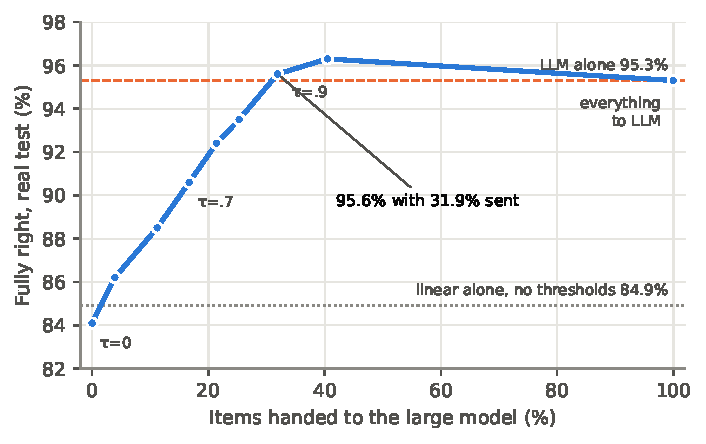
\includegraphics[width=\linewidth]{figures/fig_hybrid_handoff_curve.pdf}
    \caption{Real-test accuracy when items whose combined confidence is below $\tau$ are handed to the large language model, against the share handed off. The leftmost point is the shipped model alone with its thresholds and title bonus (84.1\%: two abstentions count as errors and the title bonus accounts for one more item); the dotted line is the unified, always-answering setting (84.9\%). Handing off about one third of items is on par with sending everything.}
    \label{fig:hybrid}
  \end{minipage}
\end{figure}

The shipped 2.1\,MB linear model is fully right on 84.9\% of the real test set (95\% interval 80.9--88.1), with 95.6\% type accuracy, 81.3\% genre accuracy and 86.2\% video-class accuracy (Table~\ref{tab:main}). The large language model, given the same four fields, reaches 95.3\% (92.7--97.0). The gap is significant: on paired items the large model is right 47 times where the linear model is wrong, against 7 the other way ($p < 0.0001$, exact McNemar). By language, the linear model is fully right on 89.9\% of English (159 items), 83.0\% of Chinese (94) and 81.4\% of Japanese titles (118); the 12 items without a language tag score 66.7\%.

A larger on-device learner does not close the gap. The transformer has 107M parameters (428\,MB in fp32, 107\,MB in int8), 50 to 200 times the linear model's file, and scores 84.1\% (80.1--87.4); averaging it with the linear model gives 86.7\% (82.9--89.7), +1.8 points or about 7 items, below the +3-point bar we set in advance for adopting it. The transformer is also clearly worse on the focus (83.1\% versus 90.3\%) and synthetic (84.7\% versus 94.9\%) sets, and dynamic int8 quantisation lowered its real-test accuracy from 84.6\% to 79.9\% (both with the shipped artist bonus). On the same 2-core CPU, the linear model takes 0.85--0.97\,ms per item in Node.js and the int8 transformer 6.6\,ms in ONNX Runtime. We trained the transformer for only 3 epochs on a CPU with frozen embeddings, so longer training may help; Section~\ref{sec:errors} suggests, however, that the errors it would need to fix are knowledge errors.

\subsection{Hybrid Hand-off}
\label{sec:handoff}

Sending only uncertain items to the large model recovers its accuracy with a third of the calls (Figure~\ref{fig:hybrid}; per-set values in Appendix Table~\ref{tab:hybrid}). At $\tau = 0.9$, 31.9\% of real-test items are handed off and the hybrid is fully right on 95.6\% (93.0--97.2), on par with sending everything (95.3\%, one item fewer). This works because the linear model's confident answers are highly accurate and the two models' errors only partly overlap. The threshold was chosen after inspecting this real-test curve; on the development split $\tau = 0.95$ is marginally better (97.2\% versus 96.9\%). In batched use the self-hosted large model took about 1\,s per request of 20 titles. The licence-clean variant reaches 94.8\% in the same scheme but hands off 44.1\% of items.



\subsection{Where the Small Model Fails}
\label{sec:errors}

\begin{figure}[t]
  \centering
  \begin{minipage}[t]{0.49\linewidth}
    \centering
    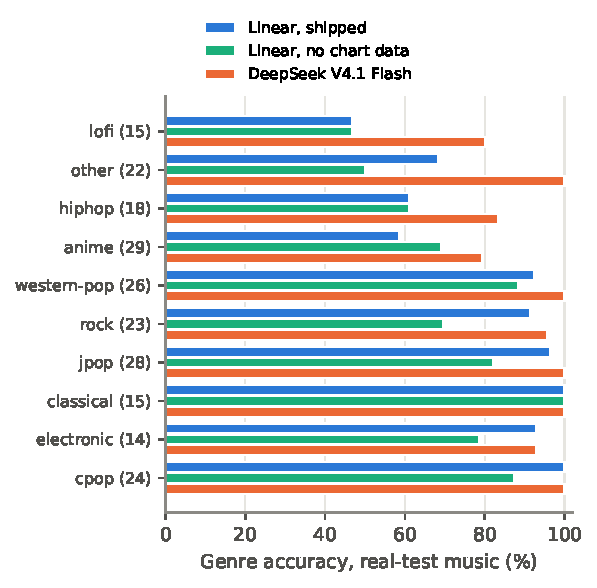
\includegraphics[width=\linewidth]{figures/fig_per_genre_accuracy_real_test.pdf}
    \caption{Per-genre accuracy on real-test music items, ordered by the gap between the large language model and the shipped linear model. The largest gaps (other, lofi, hiphop, anime) are genres that require recognising the specific artist or song.}
    \label{fig:genre}
  \end{minipage}\hfill
  \begin{minipage}[t]{0.49\linewidth}
    \centering
    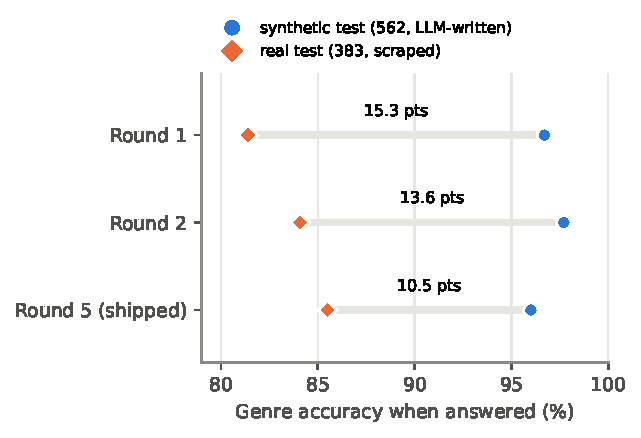
\includegraphics[width=\linewidth]{figures/fig_synthetic_vs_real_gap.pdf}
    \caption{Genre accuracy when answered on the LLM-written synthetic test split versus the scraped real test set, by development round. The synthetic set overstated real-world genre accuracy by 10.5 to 15.3 points.}
    \label{fig:synthetic}
  \end{minipage}
\end{figure}

The linear model's errors concentrate in four genres (Figure~\ref{fig:genre}): anime (58.6\% versus 79.3\% for the large model), lofi (46.7\% versus 80.0\%), hiphop (61.1\% versus 83.3\%) and other (68.2\% versus 100\%). It is at or near the large model on cpop, classical, jpop, electronic and rock. The most frequent confusions are anime songs read as jpop (5) or cpop (3), ``other'' music not recognised as music (5) and lofi read as rock (3). Anime theme songs are often sung by mainstream pop artists with no anime cue in the title, and lofi and hiphop have many new small producers.

The clearest evidence for the knowledge hypothesis comes from splitting the real-test music items by whether the system has seen the artist: the artist field or a title segment matches the artist table, or the artist appears among the music training rows (Table~\ref{tab:known}). For the 168 items with a known artist, the linear model's genre accuracy is 90.5\%, 4.7 points below the large model's 95.2\%. For the 46 items with an unknown artist it falls to 47.8\%, 39.2 points below the large model, which itself drops only 8.2 points to 87.0\%. Unknown artists make up 21\% of the music items but 24 of the linear model's 40 genre errors. Unknown-artist items may also be intrinsically harder (newer releases, fewer cues in the title), so this split supports, but does not by itself prove, the knowledge explanation.

\begin{table}[t]
  \centering
  \small
  \caption{Genre accuracy (\%) on real-test music items by whether the artist is known to the system (artist field or a title segment in the artist table, or the artist among the music training rows); unified setting, higher is better.}
  \label{tab:known}
  \begin{tabular}{@{}lrrr@{}}
    \toprule
    Artist & Items & Linear (shipped) & DeepSeek V4.1 Flash \\
    \midrule
    Known & 168 & 90.5 & 95.2 \\
    Unknown & 46 & 47.8 & 87.0 \\
    \bottomrule
  \end{tabular}
\end{table}

Targeted data helps where surface patterns exist, although we can only measure this on the LLM-written focus set. Before round 5 the training data contained 63 meme-related rows out of about 19,000; adding 1,420 meme rows, 717 idol rows with 212 group names and 907 anime rows with 352 artists raised fully-right accuracy on the focus subsets from 75.8\% to 89.2\% (memes), 85.0\% to 90.8\% (Japanese idols) and 88.3\% to 90.8\% (anime), against 93.3\%, 96.7\% and 91.7\% for the large model.

\section{Analysis and Negative Results}
\label{sec:analysis}

\subsection{Training on the Large Model's Labels Did Not Help}
\label{sec:distill}

\begin{table}[t]
  \centering
  \small
  \caption{Training the linear model on the large model's labels (real development and test combined, 637 items, no thresholds, accuracy \%; higher is better). No variant beats the model trained without teacher data.}
  \label{tab:distill}
  \begin{tabular}{@{}lrrr@{}}
    \toprule
    Variant & Genre & Video class & Type \\
    \midrule
    Round 5, no teacher data & \textbf{83.3} & \textbf{87.5} & \textbf{97.0} \\
    + 8,982 teacher rows + 286 corrections & 81.9 & 79.6 & 95.4 \\
    + 4,030 class-balanced teacher rows + corrections & \textbf{83.3} & 79.6 & 96.2 \\
    Teacher rows only & 83.1 & 84.9 & \textbf{97.0} \\
    Teacher corrections only & 82.5 & 82.9 & 96.5 \\
    \bottomrule
  \end{tabular}
\end{table}

If the gap were a matter of decision boundaries, training the small model on the large model's labels should transfer some of its advantage. We used hard labels (pseudo-labelling), as in \citet{wang2021want}, rather than the soft targets of classic distillation \citep{hinton2015distilling}, so our result does not rule out the latter. We had the large model label 16,299 unlabelled real titles (remaining chart songs, 3,845 podcast episodes, 640 music videos and trending titles) and kept the 8,982 labels with confidence at least 0.8. It also audited all 21,535 existing training rows, and the 286 rows where it disagreed with confidence at least 0.9 were dropped (hand-written rows) or relabelled (chart rows). No variant improved on the round-5 model (Table~\ref{tab:distill}): genre accuracy stayed between 81.9\% and 83.3\%, and video-class accuracy fell from 87.5\% to as low as 79.6\%.

Part of the loss had a concrete cause. In the first version about a quarter of the teacher-labelled podcast episodes were attached to a video-site host, which taught the student that items on that host can be podcasts. Capping teacher rows at 600 per genre and 1,500 podcasts restored genre accuracy but not video accuracy, and corrections hurt video accuracy more than new rows did; with only about 150 videos in these sets, some of this movement is noise. The audit itself was reassuring: the teacher disagreed confidently with 89 of 13,245 hand-written training rows (0.7\%), mostly on rock/pop and jpop/anime boundaries, against 197 of 8,290 rule-labelled chart rows (2.4\%). Our reading, consistent with Table~\ref{tab:known}, is that the teacher's advantage is specific knowledge (which band plays a song, what a meme refers to) that a 2\,MB linear model cannot absorb from a few thousand examples.

\subsection{Synthetic Evaluation and Data Ablations}
\label{sec:ablations}

\paragraph{Synthetic validation overstates accuracy.} In round 1 the synthetic test split reported 97.5\% type accuracy and 96.7\% genre accuracy when answered, which looked as if the targets were met. The only warning sign was 91.1\% genre accuracy on the 46 synthetic music rows whose artist was in neither the table nor the training data. On real titles the same model reached 81.4\%, and the gap stayed between 10.5 and 15.3 points across rounds (Figure~\ref{fig:synthetic}). Data written from the same kind of model's memory as the training data shares its blind spots, so from round 2 on decisions were made on real titles. The protocol was not fully clean, however: thresholds were tuned on the development split only (from round 3), but the ablations in this section and in Section~\ref{sec:distill} were scored on development and test combined, and $\tau$ was chosen on the test curve. The real-test numbers are therefore somewhat optimistic estimates of performance on new titles.

\paragraph{Chart data and conflicting taxonomies.} Adding store-chart data in round 3 raised synthetic scores but lowered the real test with thresholds. A no-threshold ablation on the real development and test sets showed the chart data itself helped (genre 78.6\% with it, 76.1\% without); the drop came from thresholds tuned on the 254-item development split and from the store's genre taxonomy, which for example files Japanese bands under rock. Letting curated lists overrule chart genres reduced conflicting artist genres from 471 to 72 and raised real genre accuracy to 82.8\%.

\paragraph{Licence-clean variant.} Because the chart feed's terms of use for model training were not verified, we also retrained without any chart-derived data. Real-test fully right fell from 84.9\% to 79.9\% (75.6--83.6) and genre accuracy from 81.3\% to 73.8\%. This is a significant paired difference: 28 items were right only for the shipped model and 9 only for the variant ($p = 0.0026$). The variant was slightly better on the focus (91.7\%) and synthetic (95.9\%) sets. Since the real test set was taken in the same week as the chart data, part of the shipped model's advantage is artist overlap; this mirrors real use when the artist table is refreshed from charts, but it would fade if the table went stale.

\paragraph{Capacity.} Doubling the hash table to $2^{18}$ buckets (4.19\,MB) raised real genre accuracy by about 2 points, within noise for twice the size, so it was not adopted.

\section{Limitations}
\label{sec:limitations}

The real test set is small: 383 items, of which 214 are music and about 100 are video, so differences below about 2 points are not reliable and per-genre numbers rest on 14 to 29 items each. It was not perfectly held out, since several ablations and the hand-off threshold were assessed with it (Section~\ref{sec:ablations}). Its labels were assigned by large-language-model sub-agents following the label guide, and the large language model may agree with them partly because both share similar judgements on boundary cases, so its 95.3\% may be optimistic. The study covers one task, three languages and a single day of data collection, and chart data and test titles come from the same week. We tested hard-label training on teacher outputs, not soft-target distillation, and trained the transformer briefly on a CPU with frozen embeddings. The Swift and C\# runtimes were written but not compiled or run. Finally, the genre taxonomy is coarse and tailored to one application, so absolute numbers do not transfer to other taxonomies.

\section{Conclusion}
\label{sec:conclusion}

A 2.1\,MB hashed character $n$-gram model with site rules and an artist table classifies trilingual media titles on the device in under a millisecond and is fully right on 84.9\% of real titles, against 95.3\% for a large language model reading the same text. The gap appears to be mainly one of knowledge rather than capacity: accuracy collapses on unseen artists, and neither teacher labels nor a briefly trained, much larger multilingual encoder helped, although our capacity tests were limited. The practical design is to keep the on-device model small, keep knowledge where it can be updated (an artist table refreshed from charts, and a server-side model behind a confidence gate that sees about a third of items), and to measure on real titles, because LLM-written validation data overstated genre accuracy by 10 to 15 points.

The shipped model, code, LLM-written training data, synthetic evaluation sets and evaluation scripts are released at \url{https://github.com/xingaobio/kobutai-model}, with weights and data under a non-commercial licence; a licence-clean variant trained without chart data and an in-browser demo are at \url{https://huggingface.co/xingaouk/kobutai-media-classifier}. The real-world evaluation titles and the chart data are not redistributed, so the headline numbers cannot be reproduced exactly from the release.

\section*{Disclosure of AI Assistance}

The experiments, code and figures in this work were produced by an AI coding agent (Claude, in Claude Code) working under the author's direction over seven development rounds in one day. Most training data, the synthetic validation and focus sets, and the labels of the real-world set were produced by large-language-model sub-agents, and DeepSeek V4.1 Flash served as reference and teacher as described above. The manuscript was drafted with AI assistance from the experiment records; the author takes responsibility for its content.

\bibliographystyle{plainnat}
\bibliography{refs}

\appendix
\section{Hand-off Thresholds on All Evaluation Sets}
\label{app:hybrid}

\begin{table}[h]
  \centering
  \small
  \caption{Hybrid hand-off: share of real-test items sent to the large language model and fully right (\%) on each set. $\tau = 0$ is the shipped model alone with its thresholds and title bonus, where its 0.5\% abstentions count as errors.}
  \label{tab:hybrid}
  \begin{tabular}{@{}lrrrrr@{}}
    \toprule
    Threshold $\tau$ & Sent (real test) & Real test & Real dev & Focus & Synth. \\
    \midrule
    0 (never) & 0.0 & 84.1 & 89.4 & 90.3 & 95.1 \\
    0.7 & 16.7 & 90.6 & 95.3 & 93.6 & 98.2 \\
    0.8 & 21.4 & 92.4 & 96.5 & 93.9 & 98.4 \\
    \textbf{0.9} & \textbf{31.9} & \textbf{95.6} & 96.9 & 93.6 & 99.0 \\
    0.95 & 40.5 & 96.3 & 97.2 & 94.4 & 98.9 \\
    Always & 100.0 & 95.3 & 95.3 & 93.9 & 98.3 \\
    \bottomrule
  \end{tabular}
\end{table}

\end{document}
